% Capitolul 0: Seminar - Fundamentele Seriilor de Timp
% Prezentare academică de calitate Harvard
% Program de licență, Academia de Studii Economice din București

\documentclass[9pt, aspectratio=169, t]{beamer}

% Asigură încadrarea conținutului pe diapozitive
\setbeamersize{text margin left=8mm, text margin right=8mm}

%=============================================================================
% CONFIGURARE TEMĂ ȘI STIL
%=============================================================================
\usetheme{default}
% Using default theme for clean header/footer control

% Color Palette (matching Redispatch PDF)
\definecolor{MainBlue}{RGB}{26, 58, 110}
\definecolor{AccentBlue}{RGB}{26, 58, 110}
\definecolor{IDAred}{RGB}{205, 0, 0}
\definecolor{DarkGray}{RGB}{51, 51, 51}
\definecolor{MediumGray}{RGB}{128, 128, 128}
\definecolor{LightGray}{RGB}{248, 248, 248}
\definecolor{VeryLightGray}{RGB}{235, 235, 235}
\definecolor{KeynoteGray}{RGB}{218, 218, 218}
\definecolor{SectionGray}{RGB}{120, 120, 120}
\definecolor{FooterGray}{RGB}{100, 100, 100}
\definecolor{Crimson}{RGB}{220, 53, 69}
\definecolor{Forest}{RGB}{46, 125, 50}
\definecolor{Amber}{RGB}{181, 133, 63}
\definecolor{Orange}{RGB}{230, 126, 34}
\definecolor{Purple}{RGB}{142, 68, 173}

% Gradient background (exact Keynote 315° gradient: white to RGB 218,218,218)
\setbeamertemplate{background}{%
    \begin{tikzpicture}[remember picture, overlay]
        \shade[shading=axis, shading angle=315,
        top color=white, bottom color=KeynoteGray]
        (current page.south west) rectangle (current page.north east);
    \end{tikzpicture}%
}
% Fallback solid color for compatibility
\setbeamercolor{background canvas}{bg=}

\setbeamercolor{palette primary}{bg=MainBlue, fg=white}
\setbeamercolor{palette secondary}{bg=MainBlue!85, fg=white}
\setbeamercolor{palette tertiary}{bg=MainBlue!70, fg=white}
\setbeamercolor{structure}{fg=MainBlue}
\setbeamercolor{title}{fg=IDAred}
\setbeamercolor{frametitle}{fg=IDAred, bg=}
\setbeamercolor{block title}{bg=MainBlue, fg=white}
\setbeamercolor{block body}{bg=VeryLightGray, fg=DarkGray}
\setbeamercolor{block title alerted}{bg=Crimson, fg=white}
\setbeamercolor{block body alerted}{bg=Crimson!8, fg=DarkGray}
\setbeamercolor{block title example}{bg=Forest, fg=white}
\setbeamercolor{block body example}{bg=Forest!8, fg=DarkGray}
\setbeamercolor{item}{fg=MainBlue}

% Footer colors (override Madrid theme blue)
\setbeamercolor{author in head/foot}{fg=FooterGray, bg=}
\setbeamercolor{title in head/foot}{fg=FooterGray, bg=}
\setbeamercolor{date in head/foot}{fg=FooterGray, bg=}
\setbeamercolor{section in head/foot}{fg=FooterGray, bg=}
\setbeamercolor{subsection in head/foot}{fg=FooterGray, bg=}

% Bullet styles (apply everywhere including blocks)
\setbeamertemplate{itemize item}{\color{MainBlue}$\boxdot$}
\setbeamertemplate{itemize subitem}{\color{MainBlue}$\blacktriangleright$}
\setbeamertemplate{itemize subsubitem}{\color{MainBlue}\tiny$\bullet$}
\setbeamertemplate{itemize/enumerate body begin}{\normalsize}
\setbeamertemplate{itemize/enumerate subbody begin}{\normalsize}

% Item spacing - compact style
\setlength{\leftmargini}{10pt}       % Level 1: minimal indent
\setlength{\leftmarginii}{10pt}      % Level 2: minimal additional indent
% Compact list spacing (zero extra space before/after lists in blocks)
\makeatletter
\def\@listi{\leftmargin\leftmargini \topsep 0pt \parsep 0pt \itemsep 0pt}
\def\@listii{\leftmargin\leftmarginii \topsep 0pt \parsep 0pt \itemsep 0pt}
\makeatother

\setbeamertemplate{navigation symbols}{}

%=============================================================================
% CUSTOM HEADLINE
%=============================================================================
\setbeamertemplate{headline}{%
    \vskip10pt%
    \hbox to \paperwidth{%
        \hskip0.5cm%
        {\small\color{FooterGray}\renewcommand{\hyperlink}[2]{##2}\insertsectionhead}%
        \hfill%
        \textcolor{FooterGray}{\small\insertframenumber}%
        \hskip0.5cm%
    }%
    \vskip4pt%
    {\color{FooterGray}\hrule height 0.4pt}%
}

%=============================================================================
% CUSTOM FOOTER
%=============================================================================
\usepackage{fontawesome5}

\setbeamertemplate{footline}{%
    {\color{FooterGray}\hrule height 0.4pt}%
    \vskip4pt%
    \hbox to \paperwidth{%
        \hskip0.5cm%
        \textcolor{FooterGray}{\small Analiza și Prognoza seriilor de timp}%
        \hfill%
        \raisebox{-0.1em}{%
            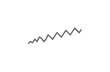
\begin{tikzpicture}[x=0.08em, y=0.08em, line width=0.4pt]
                \draw[FooterGray] (0,3) -- (1,4) -- (2,3.5) -- (3,5) -- (4,4) -- (5,6) -- (6,5.5) -- (7,4) -- (8,5) -- (9,7) -- (10,6) -- (11,5) -- (12,6.5) -- (13,8) -- (14,7) -- (15,6) -- (16,7.5) -- (17,9) -- (18,8) -- (19,7) -- (20,8.5) -- (21,10) -- (22,9) -- (23,8) -- (24,9.5);
            \end{tikzpicture}%
        }%
        \hskip0.5cm%
    }%
    \vskip6pt%
}

%=============================================================================
% PACHETE
%=============================================================================
\usepackage[utf8]{inputenc}
\usepackage[T1]{fontenc}
\usepackage[romanian]{babel}
\usepackage{amsmath, amssymb, amsthm}
\usepackage{mathtools}
\usepackage{bm}
\usepackage{tikz}
\usetikzlibrary{arrows.meta, positioning, shapes, calc, decorations.pathreplacing, shadings}
\usepackage{booktabs}
\usepackage{multirow}
\usepackage{array}
\usepackage{graphicx}
\usepackage{hyperref}
\usepackage{colortbl}
\hypersetup{colorlinks=true, linkcolor=MainBlue, urlcolor=MainBlue}
\graphicspath{{../../logos/}{../../charts/}}
\hfuzz=2pt  % Suppress tiny overfull warnings (<2pt)
\vfuzz=2pt  % Suppress tiny vertical overfull warnings (<2pt)

%=============================================================================
% COMANDA QUANTLET
%=============================================================================
\newcommand{\quantlet}[2]{%
    \hfill\href{#2}{%
        \raisebox{-0.15em}{\includegraphics[height=0.7em]{ql_logo.png}}%
        \textcolor{MainBlue}{\tiny\ #1}%
    }%
}

%=============================================================================
%=============================================================================
% CENTRED MINIPAGE (fara spatiu vertical suplimentar)
%=============================================================================
\newenvironment{cminipage}[1]{%
    \par\noindent\hfill\begin{minipage}{#1}\ignorespaces
}{%
    \end{minipage}\hfill\null\par
}


% COMENZI PERSONALIZATE
%=============================================================================
\newcommand{\E}{\mathbb{E}}
\newcommand{\Var}{\text{Var}}
\newcommand{\Cov}{\text{Cov}}
\newcommand{\Corr}{\text{Corr}}
\newcommand{\R}{\mathbb{R}}
\newcommand{\RMSE}{\text{RMSE}}
\newcommand{\MAE}{\text{MAE}}
\newcommand{\MAPE}{\text{MAPE}}

\newcommand{\correct}{\textcolor{Forest}{\checkmark}}
\newcommand{\incorrect}{\textcolor{Crimson}{\texttimes}}

%=============================================================================
% PAGINĂ TITLU PERSONALIZATĂ
%=============================================================================
\defbeamertemplate*{title page}{hybrid}[1][]
{
    \vspace{0.2cm}
    % Logos row - top header (with clickable links)
    \begin{center}
        \href{https://www.ase.ro}{\includegraphics[height=1.0cm]{ase_logo.png}}\hspace{0.3cm}%
        \href{https://theida.net}{\includegraphics[height=1.0cm]{ida_logo.png}}\hspace{0.3cm}%
        \href{https://blockchain-research-center.com}{\includegraphics[height=1.0cm]{brc_logo.png}}\hspace{0.3cm}%
        \href{https://www.ai4efin.ase.ro}{\includegraphics[height=1.0cm]{ai4efin_logo.png}}\hspace{0.3cm}%
        \href{https://ipe.ro/new}{\includegraphics[height=1.0cm]{acad_logo.png}}\hspace{0.3cm}%
        \href{https://www.digital-finance-msca.com}{\includegraphics[height=1.0cm]{msca_logo.png}}%
    \end{center}

    \vspace{0.6cm}

    % Main title with Q logos on sides (with clickable links)
    \begin{center}
        \begin{minipage}{0.1\textwidth}
            \centering
            \href{https://quantlet.com}{\includegraphics[height=1.1cm]{ql_logo.png}}
        \end{minipage}%
        \begin{minipage}{0.78\textwidth}
            \centering
            {\LARGE\bfseries\usebeamercolor[fg]{title}\inserttitle}

            \vspace{0.3cm}

            {\usebeamerfont{subtitle}\usebeamercolor[fg]{title}\insertsubtitle}
        \end{minipage}%
        \begin{minipage}{0.1\textwidth}
            \centering
            \href{https://quantinar.com}{\includegraphics[height=1.1cm]{qr_logo.png}}
        \end{minipage}
    \end{center}

    \vspace{0.6cm}

    % Authors (left aligned)
    \hspace{0.5cm}{\usebeamerfont{author}\insertauthor}

    \vspace{0.3cm}

    % Institute/Affiliations (left aligned)
    \hspace{0.5cm}\begin{minipage}[t]{0.9\textwidth}
        \raggedright\small\insertinstitute
    \end{minipage}
}

%=============================================================================
% INFORMAȚII TITLU
%=============================================================================
\title[Analiza Seriilor de Timp]{Analiza și Prognoza seriilor de timp}
\subtitle{Seminar 0: Fundamente}
\author[D.T. Pele]{Daniel Traian PELE}
\institute{Academia de Studii Economice din București\\
IDA Institute Digital Assets\\
Blockchain Research Center\\
AI4EFin Artificial Intelligence for Energy Finance\\
Academia Română, Institutul de Prognoză Economică\\
MSCA Digital Finance}
\date{}

\begin{document}

% Title page (no header/footer)
{
\setbeamertemplate{headline}{}
\setbeamertemplate{footline}{}
\begin{frame}
    \titlepage
\end{frame}
}

%=============================================================================
% CUPRINS
%=============================================================================
\begin{frame}{Cuprins Seminar}
    \begin{cminipage}{0.95\textwidth}
    \textbf{\large Structura seminarului:}

    \vspace{0.4cm}

    \begin{enumerate}
        \item[\textcolor{MainBlue}{\textbf{1.}}] \textbf{Test Grilă} -- Verificarea cunoștințelor
        \vspace{0.15cm}
        \item[\textcolor{MainBlue}{\textbf{2.}}] \textbf{Adevărat/Fals} -- Verificări conceptuale
        \vspace{0.15cm}
        \item[\textcolor{MainBlue}{\textbf{3.}}] \textbf{Exerciții de Calcul} -- Practică aplicată
        \vspace{0.15cm}
        \item[\textcolor{MainBlue}{\textbf{4.}}] \textbf{Exercițiu cu asistență AI} -- Gândire critică
        \vspace{0.15cm}
        \item[\textcolor{MainBlue}{\textbf{5.}}] \textbf{Rezumat} -- Recapitulare
    \end{enumerate}
    \end{cminipage}
\end{frame}

%=============================================================================
% TEST GRILĂ
%=============================================================================
\section{Test grilă}

\begin{frame}{Quiz 1: Bazele seriilor de timp}
    \begin{cminipage}{0.95\textwidth}
    \begin{alertblock}{Întrebare}
        Care dintre următoarele NU este o caracteristică a datelor de tip serie de timp?
    \end{alertblock}

    \vspace{0.4cm}

    \begin{block}{Variante de răspuns}
        \textcolor{MainBlue}{\textbf{(A)}} Observațiile sunt ordonate în timp\\[3pt]
        \textcolor{MainBlue}{\textbf{(B)}} Observațiile consecutive sunt de obicei corelate\\[3pt]
        \textcolor{MainBlue}{\textbf{(C)}} Observațiile sunt independente și identic distribuite\\[3pt]
        \textcolor{MainBlue}{\textbf{(D)}} Datele au o ordonare temporală naturală
    \end{block}

    \vspace{0.5cm}

    \begin{center}
        \textit{Răspunsul pe slide-ul următor...}
    \end{center}
    \end{cminipage}
\end{frame}

\begin{frame}{Quiz 1: Răspuns}
    \begin{cminipage}{0.95\textwidth}
    \begin{exampleblock}{Răspuns: C -- Observațiile sunt independente și identic distribuite}
        \textbf{Întrebare:} Care NU este o caracteristică a datelor de tip serie de timp?

        \vspace{0.3cm}

    \begin{block}{Variante de răspuns}
        \textcolor{MainBlue}{\textbf{(A)}} Observațiile sunt ordonate în timp \incorrect\\[3pt]
        \textcolor{MainBlue}{\textbf{(B)}} Observațiile consecutive sunt de obicei corelate \incorrect\\[3pt]
        \textcolor{MainBlue}{\textbf{(C)}} \textbf{\textcolor{Forest}{Observațiile sunt independente și identic distribuite}} \correct\\[3pt]
        \textcolor{MainBlue}{\textbf{(D)}} Datele au o ordonare temporală naturală \incorrect
    \end{block}

        \vspace{0.3cm}

        \begin{itemize}
            \item Observațiile seriilor de timp sunt \textbf{dependente} (autocorelate), nu independente
            \item Ipoteza i.i.d.\ este fundamentală pentru analiza transversală, dar este \textbf{încălcată} în seriile de timp
            \item Această dependență temporală necesită \textbf{metode specializate}
        \end{itemize}
    \end{exampleblock}
    
    \end{cminipage}
    \quantlet{TSA\_ch0\_definition}{https://github.com/QuantLet/TSA/tree/main/TSA_ch0/TSA_ch0_definition}
\end{frame}

\begin{frame}{Quiz 2: Descompunere}
    \begin{cminipage}{0.95\textwidth}
    \begin{alertblock}{Întrebare}
        Când ar trebui să folosiți descompunerea multiplicativă în loc de cea aditivă?
    \end{alertblock}

    \vspace{0.4cm}

    \begin{block}{Variante de răspuns}
        \textcolor{MainBlue}{\textbf{(A)}} Când modelul sezonier are amplitudine constantă\\[3pt]
        \textcolor{MainBlue}{\textbf{(B)}} Când varianța seriei este stabilă în timp\\[3pt]
        \textcolor{MainBlue}{\textbf{(C)}} Când fluctuațiile sezoniere cresc proporțional cu nivelul\\[3pt]
        \textcolor{MainBlue}{\textbf{(D)}} Când seria nu are componentă de trend
    \end{block}

    \vspace{0.5cm}

    \begin{center}
        \textit{Răspunsul pe slide-ul următor...}
    \end{center}
    \end{cminipage}
\end{frame}

\begin{frame}{Quiz 2: Răspuns}
    \begin{cminipage}{0.95\textwidth}
    \begin{exampleblock}{Răspuns: C -- Când fluctuațiile sezoniere cresc proporțional cu nivelul}
        \vspace{-0.2cm}
        \begin{center}
            \includegraphics[width=0.95\textwidth, height=0.52\textheight, keepaspectratio]{additive_vs_multiplicative.png}
        \end{center}
        \vspace{-0.2cm}
        {\footnotesize
        \begin{itemize}\setlength{\itemsep}{0pt}
            \item \textbf{Multiplicativă}: $X_t = T_t \times S_t \times \varepsilon_t$ --- amplitudinea sezonieră \textbf{scalează cu nivelul}
            \item \textbf{Aditivă}: $X_t = T_t + S_t + \varepsilon_t$ --- amplitudine constantă
        \end{itemize}
        }
    \end{exampleblock}
    
    \end{cminipage}
    \quantlet{TSA\_ch0\_decomposition}{https://github.com/QuantLet/TSA/tree/main/TSA_ch0/TSA_ch0_decomposition}
\end{frame}

\begin{frame}{Quiz 3: Netezire exponențială}
    \begin{cminipage}{0.95\textwidth}
    \begin{alertblock}{Întrebare}
        În Netezirea exponențială Simplă cu $\alpha = 0.9$, ce se întâmplă?
    \end{alertblock}

    \vspace{0.4cm}

    \begin{block}{Variante de răspuns}
        \textcolor{MainBlue}{\textbf{(A)}} Prognozele sunt foarte netede și stabile\\[3pt]
        \textcolor{MainBlue}{\textbf{(B)}} Observațiile recente au foarte puțină pondere\\[3pt]
        \textcolor{MainBlue}{\textbf{(C)}} Prognozele reacționează rapid la schimbările recente\\[3pt]
        \textcolor{MainBlue}{\textbf{(D)}} Prognoza este în esență o medie pe termen lung
    \end{block}

    \vspace{0.5cm}

    \begin{center}
        \textit{Răspunsul pe slide-ul următor...}
    \end{center}
    \end{cminipage}
\end{frame}

\begin{frame}{Quiz 3: Răspuns}
    \begin{cminipage}{0.95\textwidth}
    \begin{exampleblock}{Răspuns: C -- Prognozele reacționează rapid la schimbările recente}
        Cu $\alpha = 0.9$: $\hat{X}_{t+1} = 0.9 X_t + 0.1 \hat{X}_t$
        \begin{itemize}
            \item \textbf{$\alpha$ mare} (ex.\ 0.9): 90\% pondere pe ultima observație
                \begin{itemize}
                    \item Prognoze foarte receptive la date noi
                \end{itemize}
            \item \textbf{$\alpha$ mic} (ex.\ 0.1): prognoze mai netede, mai stabile
                \begin{itemize}
                    \item Ia în calcul mai multe observații din trecut
                \end{itemize}
        \end{itemize}
    \end{exampleblock}
    
    \end{cminipage}
    \quantlet{TSA\_ch0\_smoothing}{https://github.com/QuantLet/TSA/tree/main/TSA_ch0/TSA_ch0_smoothing}
\end{frame}

\begin{frame}{Quiz 4: Medii mobile}
    \begin{cminipage}{0.95\textwidth}
    \begin{alertblock}{Întrebare}
        Ce observații folosește o medie mobilă centrată de ordin 5 (MA-5) pentru a estima trendul la momentul $t$?
    \end{alertblock}

    \vspace{0.4cm}

    \begin{block}{Variante de răspuns}
        \textcolor{MainBlue}{\textbf{(A)}} $X_t, X_{t+1}, X_{t+2}, X_{t+3}, X_{t+4}$\\[3pt]
        \textcolor{MainBlue}{\textbf{(B)}} $X_{t-4}, X_{t-3}, X_{t-2}, X_{t-1}, X_t$\\[3pt]
        \textcolor{MainBlue}{\textbf{(C)}} $X_{t-2}, X_{t-1}, X_t, X_{t+1}, X_{t+2}$\\[3pt]
        \textcolor{MainBlue}{\textbf{(D)}} $X_{t-1}, X_t, X_{t+1}$
    \end{block}

    \vspace{0.5cm}

    \begin{center}
        \textit{Răspunsul pe slide-ul următor...}
    \end{center}
    \end{cminipage}
\end{frame}

\begin{frame}{Quiz 4: Răspuns}
    \begin{cminipage}{0.95\textwidth}
    \begin{exampleblock}{Răspuns: C -- $X_{t-2}, X_{t-1}, X_t, X_{t+1}, X_{t+2}$}
        \vspace{-0.2cm}
        \begin{center}
            \includegraphics[width=0.95\textwidth, height=0.52\textheight, keepaspectratio]{ch1_moving_average.png}
        \end{center}
        \vspace{-0.2cm}
        {\footnotesize
        \begin{itemize}\setlength{\itemsep}{0pt}
            \item \textbf{MA centrată}: folosește $(k-1)/2$ observații de fiecare parte a lui $t$
            \item \textbf{MA-5}: 2 înainte + $t$ + 2 după $\Rightarrow$ fereastră mai mare = mai neted
        \end{itemize}
        }
    \end{exampleblock}
    
    \end{cminipage}
    \quantlet{TSA\_ch0\_definition}{https://github.com/QuantLet/TSA/tree/main/TSA_ch0/TSA_ch0_definition}
\end{frame}

\begin{frame}{Quiz 5: Evaluarea prognozei}
    \begin{cminipage}{0.95\textwidth}
    \begin{alertblock}{Întrebare}
        Care metrică este cea mai potrivită pentru compararea acurateței prognozei între serii cu scale diferite?
    \end{alertblock}

    \vspace{0.4cm}

    \begin{block}{Variante de răspuns}
        \textcolor{MainBlue}{\textbf{(A)}} Eroarea Absolută Medie (MAE)\\[3pt]
        \textcolor{MainBlue}{\textbf{(B)}} Rădăcina Erorii Medii Pătratice (RMSE)\\[3pt]
        \textcolor{MainBlue}{\textbf{(C)}} Eroarea Absolută Medie Procentuală (MAPE)\\[3pt]
        \textcolor{MainBlue}{\textbf{(D)}} Eroarea Medie Pătratică (MSE)
    \end{block}

    \vspace{0.5cm}

    \begin{center}
        \textit{Răspunsul pe slide-ul următor...}
    \end{center}
    \end{cminipage}
\end{frame}

\begin{frame}{Quiz 5: Răspuns}
    \begin{cminipage}{0.95\textwidth}
    \begin{exampleblock}{Răspuns: C -- Eroarea Absolută Medie Procentuală (MAPE)}
        MAPE $= \frac{100}{n}\sum\left|\frac{e_t}{X_t}\right|$ exprimă erorile ca \textbf{procente}.

        \begin{itemize}
            \item MAE, RMSE, MSE sunt \textbf{dependente de scală} (unități ale lui $X_t$)
            \item MAPE este \textbf{independentă de scală} (întotdeauna în \%)
            \item Atenție: MAPE devine instabilă când $X_t \approx 0$
        \end{itemize}
    \end{exampleblock}
    
    \end{cminipage}
    \quantlet{TSA\_ch0\_forecast\_eval}{https://github.com/QuantLet/TSA/tree/main/TSA_ch0/TSA_ch0_forecast_eval}
\end{frame}

\begin{frame}{Quiz 6: Validare încrucișată}
    \begin{cminipage}{0.95\textwidth}
    \begin{alertblock}{Întrebare}
        De ce nu putem folosi validarea încrucișată standard k-fold pentru seriile de timp?
    \end{alertblock}

    \vspace{0.4cm}

    \begin{block}{Variante de răspuns}
        \textcolor{MainBlue}{\textbf{(A)}} Datele seriilor de timp sunt prea mici\\[3pt]
        \textcolor{MainBlue}{\textbf{(B)}} Ar încălca ordonarea temporală (viitorul prezicând trecutul)\\[3pt]
        \textcolor{MainBlue}{\textbf{(C)}} Validarea încrucișată este întotdeauna invalidă\\[3pt]
        \textcolor{MainBlue}{\textbf{(D)}} Seriile de timp nu au nevoie de validare
    \end{block}

    \vspace{0.5cm}

    \begin{center}
        \textit{Răspunsul pe slide-ul următor...}
    \end{center}
    \end{cminipage}
\end{frame}

\begin{frame}{Quiz 6: Răspuns}
    \begin{cminipage}{0.95\textwidth}
    \begin{exampleblock}{Răspuns: B -- Ar încălca ordonarea temporală}
        \vspace{-0.2cm}
        \begin{center}
            \includegraphics[width=0.95\textwidth, height=0.52\textheight, keepaspectratio]{ch8_timeseries_cv.png}
        \end{center}
        \vspace{-0.2cm}
        {\footnotesize
        \textbf{Principiu}: datele viitoare nu pot fi folosite pentru a prezice trecutul! Se recomandă CV cu fereastră mobilă/în expansiune.
        }
    \end{exampleblock}
    
    \end{cminipage}
    \quantlet{TSA\_ch0\_forecast\_eval}{https://github.com/QuantLet/TSA/tree/main/TSA_ch0/TSA_ch0_forecast_eval}
\end{frame}

\begin{frame}{Vizual: Descompunerea seriei de timp}
    \begin{cminipage}{0.95\textwidth}
    \vspace{-0.3cm}
    \begin{center}
        \includegraphics[width=0.88\textwidth, height=0.55\textheight, keepaspectratio]{ch1_decomposition.png}
    \end{center}
    \vspace{-0.3cm}
    {\footnotesize
    \begin{exampleblock}{Componentele descompunerii}
        \begin{itemize}\setlength{\itemsep}{0pt}
            \item \textbf{Trend}: mișcare pe termen lung \quad \textbf{Sezonalitate}: tipar periodic \quad \textbf{Reziduu}: zgomot aleatoriu
        \end{itemize}
    \end{exampleblock}
    }
    
    \end{cminipage}
    \quantlet{TSA\_ch0\_decomposition}{https://github.com/QuantLet/TSA/tree/main/TSA_ch0/TSA_ch0_decomposition}
\end{frame}

%=============================================================================
% ADEVĂRAT/FALS
%=============================================================================
\section{Adevărat/Fals}

\begin{frame}{Adevărat sau Fals? --- Întrebări}
    \begin{cminipage}{0.95\textwidth}
    \footnotesize
    \begin{center}
    \begin{tabular}{p{9cm}c}
        \toprule
        \textbf{Afirmație} & \textbf{A/F?} \\
        \midrule
        1. Prognozele SES sunt plate (constante pentru toate orizonturile). & ? \\[0.15cm]
        2. RMSE penalizează erorile mari mai mult decât MAE. & ? \\[0.15cm]
        3. Descompunerea multiplicativă necesită date pozitive. & ? \\[0.15cm]
        4. Un $\alpha$ mai mare înseamnă mai multă netezire. & ? \\[0.15cm]
        5. Setul de test se folosește pentru ajustarea hiperparametrilor. & ? \\[0.15cm]
        6. Naive sezonier folosește valoarea de acum un sezon. & ? \\[0.15cm]
        7. MAPE poate fi infinit dacă valorile reale sunt zero. & ? \\
        \bottomrule
    \end{tabular}
    \end{center}
    \end{cminipage}
\end{frame}

\begin{frame}{Adevărat sau Fals? --- Răspunsuri}
    \begin{cminipage}{0.95\textwidth}
    \scriptsize
    \begin{center}
    \begin{tabular}{p{7.5cm}cc}
        \toprule
        \textbf{Afirmație} & \textbf{A/F} & \textbf{Explicație} \\
        \midrule
        1. Prognozele SES sunt plate (constante pentru toate orizonturile). & \textcolor{Forest}{\textbf{A}} & {\tiny Fără trend} \\[0.08cm]
        2. RMSE penalizează erorile mari mai mult decât MAE. & \textcolor{Forest}{\textbf{A}} & {\tiny Erori pătratice} \\[0.08cm]
        3. Descompunerea multiplicativă necesită date pozitive. & \textcolor{Forest}{\textbf{A}} & {\tiny Nu se poate $\times$ negativ} \\[0.08cm]
        4. Un $\alpha$ mai mare înseamnă mai multă netezire. & \textcolor{Crimson}{\textbf{F}} & {\tiny $\alpha$ mare = mai puțin neted} \\[0.08cm]
        5. Setul de test se folosește pentru ajustarea hiperparametrilor. & \textcolor{Crimson}{\textbf{F}} & {\tiny Folosiți validare!} \\[0.08cm]
        6. Naive sezonier folosește valoarea de acum un sezon. & \textcolor{Forest}{\textbf{A}} & {\tiny $\hat{X}_{t+h} = X_{t+h-m}$} \\[0.08cm]
        7. MAPE poate fi infinit dacă valorile reale sunt zero. & \textcolor{Forest}{\textbf{A}} & {\tiny Împărțire la zero} \\
        \bottomrule
    \end{tabular}
    \end{center}
    \end{cminipage}
\end{frame}

%=============================================================================
% EXERCIȚII DE CALCUL
%=============================================================================
\section{Exerciții de calcul}

\begin{frame}{Exercițiu 1: Netezire Exponențială Simplă}
    \begin{cminipage}{0.95\textwidth}
    \begin{alertblock}{Problemă}
        \begin{itemize}\setlength{\itemsep}{0pt}
            \item \textbf{Date}: $X = [10, 12, 11, 14, 13]$ cu $\alpha = 0.3$, $\hat{X}_1 = 10$
            \item \textbf{Calculați}: a) Prognozele $\hat{X}_2$ până la $\hat{X}_6$; b) MAE și RMSE
            \item \textbf{Formula}: $\hat{X}_{t+1} = \alpha X_t + (1-\alpha)\hat{X}_t$
        \end{itemize}
    \end{alertblock}

    \vspace{0.2cm}
    \begin{exampleblock}{Soluție}
        \begin{center}
        \small
        \begin{tabular}{c|ccccc|c}
            $t$ & 1 & 2 & 3 & 4 & 5 & 6\\
            \hline
            $X_t$ & 10 & 12 & 11 & 14 & 13 & ?\\
            $\hat{X}_t$ & 10 & 10 & 10.6 & 10.72 & 11.70 & \textbf{12.09}\\
        \end{tabular}
        \end{center}
        \begin{itemize}\setlength{\itemsep}{0pt}
            \item \textbf{MAE} $= 1.745$ \quad \textbf{RMSE} $= 2.04$
        \end{itemize}
    \end{exampleblock}
    \end{cminipage}
\end{frame}

\begin{frame}{Exercițiu 2: Metrici de eroare}
    \begin{cminipage}{0.95\textwidth}
    \begin{alertblock}{Problemă}
        \begin{itemize}\setlength{\itemsep}{0pt}
            \item \textbf{Date}: $X = [100, 110, 105, 120]$, $\hat{X} = [95, 108, 110, 115]$
            \item \textbf{Calculați}: MAE, MSE, RMSE, MAPE
        \end{itemize}
    \end{alertblock}

    \vspace{0.2cm}
    \begin{exampleblock}{Soluție}
        \begin{itemize}\setlength{\itemsep}{0pt}
            \item \textbf{Erori}: $e = [5, 2, -5, 5]$
            \item \textbf{MAE} $= (|5|+|2|+|-5|+|5|)/4 = 4.25$
            \item \textbf{MSE} $= (25+4+25+25)/4 = 19.75$
            \item \textbf{RMSE} $= \sqrt{19.75} = 4.44$
            \item \textbf{MAPE} $= 25 \times (0.05+0.018+0.048+0.042) = 3.95\%$
        \end{itemize}
    \end{exampleblock}
    \end{cminipage}
\end{frame}

\begin{frame}{Exercițiu 3: Indici sezonieri}
    \begin{cminipage}{0.95\textwidth}
    \begin{alertblock}{Problemă}
        \begin{itemize}\setlength{\itemsep}{0pt}
            \item \textbf{Date}: Indici sezonieri: $S = [0.85, 1.05, 0.90, 1.20]$, Trend T4: $T = 1000$
            \item \textbf{Calculați}: a) Verificați normalizarea. b) Prognoza T4. c) Desezonalizați $X_{T4} = 1150$
        \end{itemize}
    \end{alertblock}

    \vspace{0.2cm}
    \begin{exampleblock}{Soluție}
        \begin{itemize}\setlength{\itemsep}{0pt}
            \item \textbf{a) Normalizare}: $\sum S_i = 0.85+1.05+0.90+1.20 = 4.00$ \checkmark
            \item \textbf{b) Prognoză}: $\hat{X}_{T4} = 1000 \times 1.20 = \textbf{1200}$
            \item \textbf{c) Desezonalizare}: $X_{desezonalizat} = 1150/1.20 = \textbf{958.33}$ (sub trend)
        \end{itemize}
    \end{exampleblock}
    \end{cminipage}
\end{frame}

%=============================================================================
% EXERCIȚIU CU ASISTENȚĂ AI
%=============================================================================
\section{Exercițiu cu asistență AI}

\begin{frame}{Exercițiu AI: Gândire critică}
    \begin{cminipage}{0.95\textwidth}
    \vspace{-0.3cm}
    \begin{block}{\footnotesize Prompt de testat în ChatGPT / Claude / Copilot}
        {\footnotesize
        ``Folosind yfinance, descarcă datele SPY. Descompune seria și prognozează anul viitor cu netezire exponențială. Care model e cel mai bun? Arată-mi rezultatele.''
        }
    \end{block}
    \vspace{-2mm}
    {\footnotesize
    \textbf{Exercițiu}:
    \begin{enumerate}\setlength{\itemsep}{0pt}
        \item Rulați prompt-ul într-un LLM la alegere și analizați critic răspunsul.
        \item AI alege descompunere aditivă sau multiplicativă? Alegerea e justificată?
        \item Cum evaluează modelele --- folosește RMSE pe antrenare sau pe test?
        \item Verificați parametrii de netezire ($\alpha$, $\beta$, $\gamma$). Valori aproape de 1{,}0 sunt problematice?
        \item Codul împarte corect datele în antrenare/test, sau evaluează pe date de antrenare?
    \end{enumerate}
    }
    \vspace{-2mm}
    \begin{alertblock}{}
        {\footnotesize \textbf{Atenție}: Codul generat de AI poate rula fără erori și arăta profesional. \textit{Asta nu înseamnă că e corect.}}
    \end{alertblock}
    \end{cminipage}
\end{frame}

%=============================================================================
% SFÂRȘIT
%=============================================================================
\section{Rezumat}

\begin{frame}{Rezumat: Capitolul 0}
    \begin{cminipage}{0.95\textwidth}
    \begin{exampleblock}{Concepte cheie}
        \begin{itemize}\setlength{\itemsep}{2pt}
            \item[\textcolor{MainBlue}{\textbf{1.}}] \textbf{Serii de timp}: observații ordonate temporal, cu dependență (autocorelație)
            \item[\textcolor{MainBlue}{\textbf{2.}}] \textbf{Descompunere}: aditivă ($X_t = T_t + S_t + \varepsilon_t$) vs multiplicativă ($X_t = T_t \times S_t \times \varepsilon_t$)
            \item[\textcolor{MainBlue}{\textbf{3.}}] \textbf{Netezire exponențială}: SES, Holt, Holt-Winters --- parametrul $\alpha$ controlează reactivitatea
            \item[\textcolor{MainBlue}{\textbf{4.}}] \textbf{Evaluarea prognozei}: MAE, RMSE, MAPE --- alegerea depinde de context
            \item[\textcolor{MainBlue}{\textbf{5.}}] \textbf{Sezonalitate}: indici sezonieri, prognoză și desezonalizare
        \end{itemize}
    \end{exampleblock}

    \vspace{0.5cm}
    \begin{center}
        \Large\textcolor{MainBlue}{Întrebări?}
    \end{center}
    \end{cminipage}
\end{frame}


%=============================================================================
% BIBLIOGRAFIE (aceleași referințe ca în curs)
%=============================================================================
\section{Bibliografie}

\begin{frame}{Bibliografie I}
    \begin{cminipage}{0.95\textwidth}
    \begin{block}{Fundamente ale seriilor de timp}
        {\small
        \begin{itemize}\setlength{\itemsep}{0pt}
            \item Hyndman, R.J., \& Athanasopoulos, G. (2021). \textit{Forecasting: Principles and Practice}, 3rd ed., OTexts.
            \item Shumway, R.H., \& Stoffer, D.S. (2017). \textit{Time Series Analysis and Its Applications}, 4th ed., Springer.
            \item Brockwell, P.J., \& Davis, R.A. (2016). \textit{Introduction to Time Series and Forecasting}, 3rd ed., Springer.
        \end{itemize}
        }
    \end{block}

    \begin{exampleblock}{Serii de timp financiare}
        {\small
        \begin{itemize}\setlength{\itemsep}{0pt}
            \item Tsay, R.S. (2010). \textit{Analysis of Financial Time Series}, 3rd ed., Wiley.
            \item Franke, J., Härdle, W.K., \& Hafner, C.M. (2019). \textit{Statistics of Financial Markets}, 4th ed., Springer.
        \end{itemize}
        }
    \end{exampleblock}
    \end{cminipage}
\end{frame}

\begin{frame}{Bibliografie II}
    \begin{cminipage}{0.95\textwidth}
    \begin{block}{Abordări moderne și Machine Learning}
        {\small
        \begin{itemize}\setlength{\itemsep}{0pt}
            \item Nielsen, A. (2019). \textit{Practical Time Series Analysis}, O'Reilly Media.
            \item Petropoulos, F., et al. (2022). \textit{Forecasting: Theory and Practice}, International Journal of Forecasting.
            \item Makridakis, S., Spiliotis, E., \& Assimakopoulos, V. (2020). The M4 Competition, International Journal of Forecasting.
        \end{itemize}
        }
    \end{block}

    \begin{exampleblock}{Resurse online și cod}
        {\small
        \begin{itemize}\setlength{\itemsep}{0pt}
            \item \textbf{Quantlet}: \url{https://quantlet.com} --- Repository de cod pentru statistică
            \item \textbf{Quantinar}: \url{https://quantinar.com} --- Platformă de învățare metode cantitative
            \item \textbf{GitHub TSA}: \url{https://github.com/QuantLet/TSA/tree/main/TSA_ch0} --- Cod Python pentru fiecare capitol
        \end{itemize}
        }
    \end{exampleblock}
    \end{cminipage}
\end{frame}

\begin{frame}{}
    \begin{cminipage}{0.95\textwidth}
    \centering
    \Huge\textcolor{IDAred}{Vă mulțumim!}

    \vspace{1cm}

    \Large\textcolor{MainBlue}{Întrebări?}

    \vspace{0.8cm}

    \normalsize
    Materialele seminarului sunt disponibile la: \url{https://danpele.github.io/Time-Series-Analysis/}

    \vspace{0.2cm}

    \href{https://quantlet.com}{\raisebox{-0.15em}{\includegraphics[height=0.8em]{ql_logo.png}} Quantlet} \hspace{0.5cm}
    \href{https://quantinar.com}{\raisebox{-0.15em}{\includegraphics[height=0.8em]{qr_logo.png}} Quantinar}
    \end{cminipage}
\end{frame}

\end{document}
